\chapter{Techniques}\label{chap:techniques}

This chapter explains the algorithms and techniques used in the analysis, and why they were chosen. Feature selection and anomaly/novelty detection techniques are discussed. The following list was created to use as a guideline to pick among possible algorithms.

\begin{itemize}
    \item Explore the possibility to detect the anomalies/novelties connected to the reported control problems with the pelton needles, by using only the process signals from the needles  
    % \item Discuss the issue with uneven sample frequency for different signals, mention different techniques for interpolation of missing data, is this a good option? why or why not? 
    \item Look at different methods for unsupervised feature selection. The datasets holds many signals, which ones can hold vital information for the needle control problem? 
    \item Look at different methods for supervised feature selection, using the RMSE between the pairwise needles as a target variable. 
    \item Analyze the features selected in the two different techniques, are they similar? If not, what seems to be the main difference between the two techniques? 
    \item use principal component analysis (PCA) and kernel PCA to reduce the number of features by linear an non linear combinations of the original feature set. Create a reduced data-matrix based on the principal components which again can be used as input for the machine learning algorithms. 
    \item Look into anomaly/novelty detection comparing the performance of different algorithms, on the different feature sets. The following list is a suggestion to algorithms, at least two should be used. Compare the algorithms in regards of performance, complexity, run-time, etc. 
    \begin{itemize}
        \item One class support vector machine
        \item Density based anomaly detection, k-nearest neighbors
        \item Clustering based anomaly detection, k-means clustering 
        \item Neural Networks 
    \end{itemize}
    \item Explain necessary steps to enable the use of the techniques in power plants, what are the challenges? What needs to be overcome before the results can be incorporated into any power plant using pelton turbines?     
    
\end{itemize}


\section{Feature selection}\label{sec:feature_selec}
    The dataset presented in chapter \ref{cha:data} is a large dataset, it contains data from a period of four years, and holds a total of $251$ process variables or features. Analyzing a dataset with $251$ features is not a trival task. Interpreting and visualizing data of such high dimensions is almost impossible. The feature size also introduces issues regarding memory and algorithm runtime, \cite{Guyon2003} and \cite{Dy2004}. Reducing the complexity of the problem is heavily correlated with reducing the number of features. Even if the main goal of this thesis is to investigate techniques for early anomaly/novelty detection, understanding how and why the algorithms work, and what it is in the data that enables them to trace an anomaly earlier than the current techniques is also very desirable. Not only introducing smarter condition monitoring but also learning more about unknown plant dynamics which can help us understand why some components fail while other does not is very desirable. 
    
    "The problem is that not all features are important. Some of the features may be redundant, some may be irrelevant, and some can even misguide clustering results" from \cite{Dy2004} sums up one of the issues with large dataset like this. A concrete example of this is shown in figure \ref{fig:feature_selection}, her one can clearly see that $X_2$ does not provide any information on how the datapoints are clustered. Including this feature in a learning algorithm does not provide any information about the two classes of data found in the dataset, hence in best case the performance will be the same as if only $X_1$ was used.  
    
    \begin{figure}
        \centering
        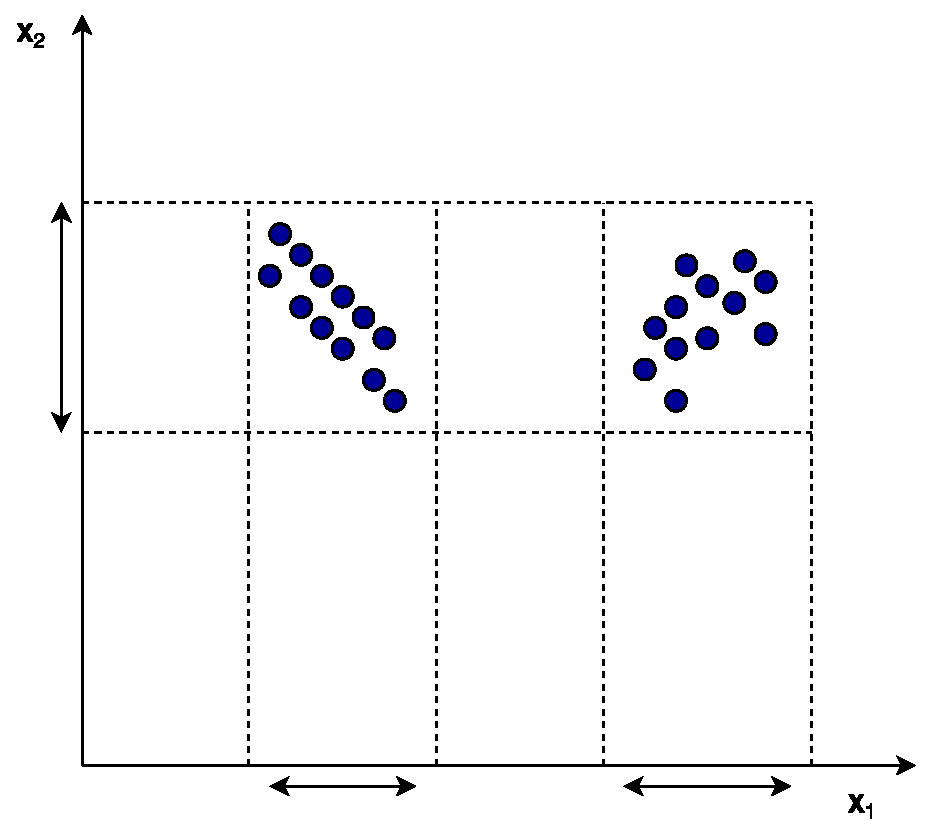
\includegraphics[width=0.5\textwidth]{report/figures/techniques/feature_selection.pdf}
        \caption{Example of a two-dimensional dataset, with one relevant and one irrelevant feature}
        \label{fig:feature_selection}
    \end{figure}
    
    
    There are two main techniques for reducing the feature size, feature selection, and dimensional reduction. The former, tries to remove the least informative and the redundant features from the feature set. The latter creates new features either as linear or non-linear combinations of the original feature set, hence one can remove the dimensions which brings litle data variance to the table. Feature selection is again separated into supervised and non-supervised selection. In the supervised case, one have a set of features and a target variable, hence one want to keep the features that is related to the target variable. For unsupervised feature selection, there is no target variable to help remove uninformative or redundant features, there is no way to confirm that the best subset of features are selected, and this area is not researched as much as the supervised case. \cite{Liu2010} states that some features can be removed without lowering the performance of a learning algorithm. 
    
    \subsection{Filter, wrapper and embedded methods}\label{subsec:filter_wrapper_embedded}
    The different classes or types of methods for feature reduction are split into three groups. This section will give a short introduction to each of them, but only filter methods will be used in this thesis.
    According to \cite{Liu2010} filter methods are methods that perform feature selection separate from the learning algorithm, and hence can be used no matter which learning algorithm is applied later. The wrapper methods however, need a predetermined learning algorithm. The features are then selected based upon the performance of the chosen algorithm.  Finally the embedded methods incorporate the selection of features in the training of the learning algorithms model.
    \cite{Liu2010} also states that since the filter methods are independent from the learning algorithm they are not biased with regard of the algorithm. Since different feature sets selected by different methods are to be tested on the same learning algorithms, this is seen as beneficial, and hence only filter methods are used in this thesis. 

\section{Supervised feature selection}\label{sec:sup_feat_select}
    As seen in chapter \ref{cha:data} the control problems with the needles can be observed in the difference or the RMSE between the pairwise controlled needles. Using the RMSE between the needles as a target variable enables the use of supervised feature selection algorithms. 
    
    
    \subsection{K-best using correlation and  mutual information}\label{subsec:K-best_feat_select}
    
        Mutual information, \cite{Kraskov2004} and \cite{Peng2005} explains how dependent or inversely how independent two variables are. It gives an understanding on how much knowing something about one variable reduces the uncertainty about the other. If two variables are completely independent, their corresponding mutual information or MI will be zero. 
        
        \begin{align}\label{eq:tech_MI}
                MI(X,Y) = \int \int p(x,y) \log \frac{p(x,y}{p_x(x),p_y(y)}
        \end{align}
        
        where $x$ and $y$ are the two variables to compare, and $p(x)$ and $py(y)$ is their corresponding probability density functions. One benefit from MI is that does not only find linear correlation between two variables, in other words it finds dependencies between variables not necessarily shown in correlation, meaning that this serves as complementary technique to using co-variance or correlation for feature selection, \cite{Li}. The K features with highest MI will be chosen. 
        
        
        The K-best features can also be selected using the correlation between a feature and the target variable. It is found as  
        \begin{align}
            corr(X,Y) = \frac{cov(X,Y}{\sigma_x\sigma_y} = \frac{E[(X-\mu_x)(Y-\mu_y)]}{\sigma_x\sigma_y}.
        \end{align}
        Here the K features with highest correlation with the target variable will be chosen. 
        
\section{Unsupervised feature selection}\label{sec:unsup_feat_reduc}
    Unsupervised feature selection is harder than supervised feature selection. The lack of a target variable, removes the ability to easily interpret which variable dynamics that are important. Still the need to reduce the feature set is prominent. \cite{Dy2004} describes the problem as follows, "The goal of feature selection for unsupervised learning is to find the smallest feature subset that best uncovers “interesting natural” groupings (clusters) from data according to the chosen criterion". The chosen criterion defines what is thought to be interesting natural groupings. As they go on to explain, there is no one optimal golden rule for defining this criterion, and a subset that is good for one purpose might not be relevant for others. The two methods chosen for unsupervised feature selection follows. \cite{He2005} states that feature selection based on data variance is one of the simplest evaluation methods, and hence it is a natural element of the analysis. 
    
    
    \subsection{Variance threshold}\label{subsec:var_thres}
    
        One of the drawbacks with using variance to select features, is that there might be a lot of features with large variances that is non-informative with what one is looking for. The algorithm is very simple, it returns the k features that has the highest variance. 
        
    
    \subsection{Laplacian score}\label{subsec:lapl_score}
        Laplacian score for feature selection was proposed as an alternative to unsupervised feature selection by \cite{He2005}. The method builds upon the assumption that features belonging to the same class or grouping will be close. The features are evaluated based on how well locality is preserved, which is found by the Laplacian score. The Laplacian score is calculated for each feature. A short introduction to the method is described below, more details can be found in \cite{He2005}. 
        
        Laplacian score is based on Laplacian Eigenmaps \cite{laplcian score for feature selection}, which is an algorithm for dimensionality reduction. The algorithm creates a nearest neighbors graph with a node for each sample of each feature. Hence the dimension becomes $m$x$\#features$. Two nodes share an edge if they are among the k-nearest neighbors to each other, meaning that k is one of they tunable parameters for this algorithm. Each edge is then given a weight based on the Gaussian radial basis function;
        
        \begin{align}\label{eq:tech_LS}
            W_{i,j} = e^-{\frac{||{\bm{X_i}-\bm{X_j}}^2||}{t}},
        \end{align}
        
        where t is another tunable parameter. Then a graph Laplacian is computed which then again is used to calculate a Laplacian score. As mentioned the algorithm has two tunable parameters. The main reson for choosing Laplacian score as one of the unsupervised feature selection methods, is that it has the ability to compare and rate features against each other. This introduces a new dimension compared to the more naive variance threshold algorithm, that only looks at one feature at a time. 
    

\section{Dimensionality reduction}\label{sec:dim_red}
    One of the issues with feature reduction is that the features that are removed, may hold information that could help the learning algorithm. In dimensional reduction, the feature set is used to create new features which means that a new reduced feature space of dimension n can hold the same amount of information as the original feature space of size m, $m>n$.

    \subsection{PCA}\label{subsec:PCA}
        Principal component analysis, is one popular technique used for dimensional reduction. PCA is an orthogonal transformation that takes a set of possibly correlated variables, and transforms them into a set of non correlated components, effectivly reducing the dimensions of the data. These new dimensions are known as principal components. There are several different algorithms that can be used to calculate the principal components, one of them is singular value decomposition or SVD. SVD decomposed the data into eigenvalues and eigenvectors. The larger a eigenvalue is, the better its corresponding eigenvector capture the variance of the data. All eigenvectors are orthogonal, this means that each vector introduces an entirely new dimension. In a high dimensional dataset with many features, there will most likely be features that are fairly similar. Figure \ref{fig:tech:PCA} shows intuitively how the PCA algorithm works. Data samples from a dataset with three features are shown in the plot. As the principal components in red and green shows, most of the variance in the samples can be represented using only one dimension. Adding the second dimension, only small residuals might be left. This illustrates how the PCA algorighm operates. 
        
        \begin{figure}
            \centering
            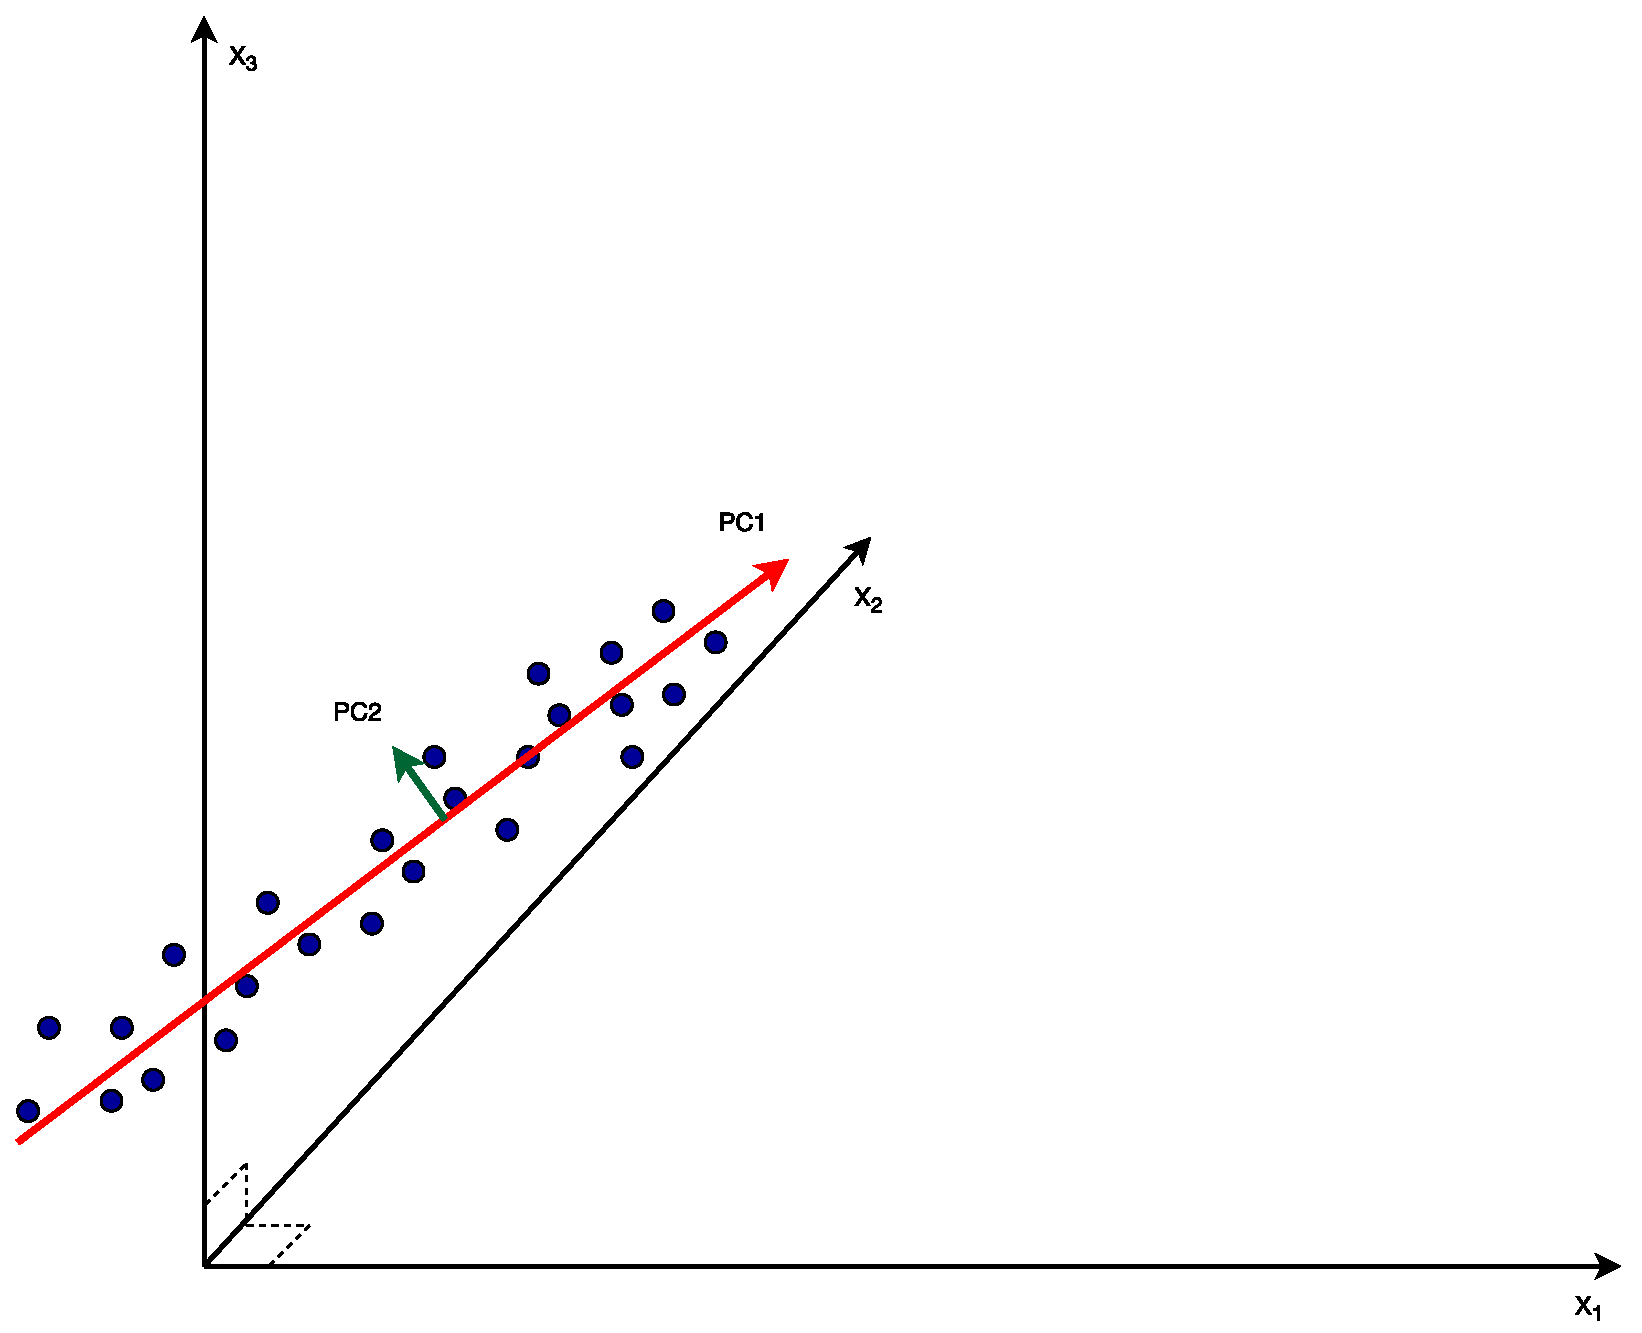
\includegraphics[width=\textwidth]{report/figures/techniques/PCA.pdf}
            \caption{Illustration on how principal component analysis work}
            \label{fig:tech:PCA}
        \end{figure}
        
    
    \subsection{Kernel PCA}\label{subsec:kernelPCA}
        Kernel PCA builds upon the PCA algorithm explained above, but it introduces a new trick. Where PCA is only able to create new features from linear combinations of the original feature set, kernel PCA uses the kernel trick to enable non-linear combinations as well. Say you have a two dimensional dataset containing samples from two different classes.  These classes are only linearly separable if the classes can be separated by a line. If one class surrounds the other class, there is no way to linearly separte the two clases in two dimensions. However, by extending the sample space into three dimensions, it might now be possible to separte the two classes with a hyperplane. Hence making a non-linear separation of the two classes possible, by still using linear methods. If the datasets are large, transforming all samples into a higher dimension can become computationally heavy. The kernel trick solves this problem without having to transform the samples. The kernel PCA extends the original PCA to a higher dimension using the kernel trick, enabling the extraction of nonlinear components.  
    
        By mapping the original data nonlinearly into a new feature space $F$ $\phi(\bm{x_1})$, and by performing PCA in this new feature space, one can get nonlinear principal components.

\section{Anomaly detection}\label{sec:Anomaly_detection}
    
    \subsection{One class SVM}\label{subsec:OCSVM}
    
            The following section is a summary based on my project thesis written the fall of 2017.
            
            Support vector machine or SVM, can be used for both supervised and unsupervised learning. In the unsupervised case, it is most commonly used for outlier and boundary detection. For supervised learning it handles two classes at a time, so one vs the rest is used if there are more than two classes. The classifier defines a hyperplane that separates the two different classes. The hyperplane can then later be used to predict which class a new feature vector belongs to.  
            
            SVM is capable of separating data both linearly and nonlinearly. How the algorithm separates the data depends on the kernel function it uses. A kernel function, or a similarity function, describes how similar two feature vectors are by taking the inner product of the two samples in a higher dimensional space. The kernel function does this without having to explicitly transform the data into this dimension.
            
            Two commonly used kernels are the Gaussian kernel
            \begin{align}
                K_g(\bm x^{1},\bm x^{2}) = e^{\frac{\norm{\bm x^{1}-\bm x^{2}}^2}{2\sigma^2}}, 
                \label{svm:gauss}
            \end{align}
            and the polynomial kernel
            \begin{align}
                K_p(\bm x^{1},\bm x^{2}) = (\bm x^{1T}\bm x^{2} + \alpha)^\beta.
                \label{svm:poly}
            \end{align}
            
            is another example of a kernel function. These are just two of many examples. The Gaussian or RBF kernell is a good first choice if you know that you have a nonlinear boundary, but don't know exactly what shape the boundary will take. If you have more knowledge about the shape of the boundary you are looking for, you might want to consider more special kernels.
    
            
            One of the great benefits of the SVM algorithm is that the solution is found by Lagrangian optimization problem 
             \begin{align}
                L = \sum_{i=1}^n  \alpha_i - \frac{1}{2} \sum_{i=1}^n \sum_{j=1}^n \alpha_i \alpha_j y^i y^j \bm x^{iT} \bm x^j,
                \label{svm:dual}
            \end{align}
            which is a convex optimization problem, and hence it has a global maxima.
            
            
            If your classes are not linearly separable in the feature space, maximization of Equation \ref{svm:dual} has no global solution. However as can be seen in Equation \ref{svm:dual} one want to minimize $\bm x_i^T  \bm x_j$. This term can then be replaced by one of the kernel functions defined above, which now enables separation in a higher dimensional space.
            
            The final thing to remark is that not all datasets are completely separable, to deal with this a slack variable is introduced into the optimization to allow miss-classification of some of the feature vectors. 
        
    
        One issue with one class svm combined with non labeled data, is that hyperparameterization becomes hard. There is no out of the box scoring function that tell you how well the classifier is performing. As long as one is working in two or three dimensions it is possible to plot the decision boundary, and select parameterization based on visual observations. In higher dimensions this becomes a proble, therefor a new method is proposed used to reduce the number of hyperparameterizations to consider. A score is given each of the paramterization from
        
        \begin{align}
            score = \abs\sigma + \mu + 100\frac{outliers}{inliers},
        \end{align}
        where the lower the score, the better the performance. $\sigma$ here represents the standard deviation of the distances from the decision boundary, $\mu$ is the unsigned distance to the decision boundary. These values were picked because the training data is said to be normal operation, and should not contain any outliers. However, this leads to the risk of a to general boundary where the classifier is no longer able to predict outliers. This means that the closer the boundary is to the samples in the training data, the higher the score. The final fraction of outliers and inliers is added to make sure that most of the data is classified as inliers. If not on runs the risk of fitting av very complex boundary which yields good distance measures for all samples, this will however lead to a large fraction of outliers which is not the case for the normal training data. 
        
        
    
    \subsection{Neural Networks}\label{subsec:NN}
    
    \subsection{K-nearest neigbours}\label{subsec:k_neig}
    
    \subsection{K-means clustering}\label{subsec:k_means}
    